\documentclass[10pt,twocolumn,letterpaper]{article}
\usepackage[margin=0.7in,columnsep=0.24in]{geometry}
\usepackage[T1]{fontenc}
\usepackage{lmodern,microtype,amsmath,amssymb,booktabs,tabularx,url,graphicx}
\usepackage[font=small,labelfont=bf]{caption}
\usepackage[hidelinks]{hyperref}
\setlength{\emergencystretch}{1em}
\widowpenalty=10000
\clubpenalty=10000
\brokenpenalty=10000
\setlength{\textfloatsep}{12pt plus 2pt minus 2pt}
\setlength{\intextsep}{10pt plus 2pt minus 2pt}
\renewcommand{\dbltopfraction}{0.95}
\renewcommand{\textfraction}{0.05}
\renewcommand{\dblfloatpagefraction}{0.7}
\title{BridgeFinder: Finding Research Collaborators\\Across Communities at UIUC}
\author{Evan Lin \qquad Eric Liu\\University of Illinois Urbana-Champaign}
\date{CS 470 Mid-Semester Report, October 2026}
\begin{document}
\raggedbottom
\maketitle

\begin{abstract}
Students often look for research opportunities through people they already know. BridgeFinder helps them look beyond those circles. A student selects a familiar researcher, explores a collaboration map, and sees related researchers with possible introduction paths. At midterm, we have built the web prototype, analyzed two UIUC publication datasets, and gathered feedback from five students. A test using past collaborations finds better predictions than shared-contact ranking, although the gains fall short of our goals. Next, we will test whether students find the suggestions relevant, unfamiliar, and useful for contacting someone.
\end{abstract}

\section{Objective}
A student who enjoyed a computing class might want to apply those skills in biology or agriculture. The difficult part is often knowing whom to approach. The student may know their instructor but have few connections outside the department. Searching by keyword can return relevant names without explaining how to start a conversation.

\textbf{BridgeFinder} finds researchers with related interests outside a familiar researcher's collaboration group and shows who might connect them. We focus on UIUC undergraduate and early-stage graduate students looking for research opportunities beyond their current department. A student can begin with an instructor or researcher whose work they know, without needing publications of their own.

The main design challenge is to balance relevance with discovery. A suggestion should match the student's interests while adding someone they would be unlikely to find through their usual contacts. It should also explain a practical next step. At midterm, we have a working three-screen app, a pipeline for building the collaboration graph, tests on two publication datasets, and one round of student feedback. Our results show promise for finding later collaborators; whether the app helps students find mentors remains an open question.

\section{Related Work}
\textbf{Researcher search.} Illinois Experts~\cite{experts} brings together institutional profiles and publications, making it a useful place to check someone's expertise. Google Scholar~\cite{scholar} supports publication search and author profiles, which help a student follow a research topic. Both are useful sources of candidate names. Our task goes a step further: explain how a candidate relates to someone the student already knows. We therefore put the collaboration map and possible introduction beside the research match, rather than expecting a profile search to answer that question.

\textbf{Literature maps.} Connected Papers~\cite{connectedpapers} gives a visual overview of related papers, helping a reader get oriented in an unfamiliar area. ResearchRabbit~\cite{researchrabbit} supports exploring related literature from a collection of papers. Their strength is making discovery an exploration rather than a sequence of keyword searches. For our purpose, however, a route between papers is not an introduction between people. BridgeFinder borrows the map-based interaction but makes researchers, shared co-authors, and candidate explanations the main objects.

\textbf{Collaboration recommendation.} Liben-Nowell and Kleinberg~\cite{libennowell2007} compare ways to predict future links from a network. Common-neighbor measures such as Adamic--Adar are simple, explainable comparisons, but favor people who already share contacts. We retain shared contacts as useful routes while restricting candidates to another community. Tang et al.~\cite{tang2012} address cross-domain collaboration recommendation using evidence about research interests and relationships. Their strength is treating relevance across domains as a recommendation problem. That ranking task does not by itself test whether a student can understand a suggested contact or use an introduction path. Our study therefore measures relevance, novelty, and willingness to contact someone, alongside the prediction test.

\textbf{Evidence about research networks.} Granovetter~\cite{granovetter1973} explains how weak ties can carry information beyond close circles; Burt~\cite{burt1992,burt2004} explains the benefits available to people who bridge separate groups. These works give us a reason to look across communities, but they do not establish the value of a particular missing co-authorship. Dahlander and McFarland~\cite{dahlander2013} study how research ties form and persist over time, showing why intellectual similarity and organizational context matter. That longitudinal view helps explain collaboration, but does not provide our student-facing discovery workflow. BridgeFinder turns these ideas into suggestions that can be explored; publication data alone still cannot establish personal trust or mentoring availability.

\section{Network Analysis}
\subsection{Building the graph}
We use OpenAlex~\cite{openalex} publications from 2015--2024. Each node represents an author affiliated with UIUC on a collected paper. Two authors share an edge if they wrote a paper together. We keep papers with at least two UIUC authors and omit collaborators outside UIUC.

We collected a pilot sample of 5,000 works and a larger sample of 25,000 works. After keeping papers with multiple UIUC authors, these contain 2,493 and 13,229 papers, respectively. They are samples of campus research, not a complete directory. Table~\ref{tab:network} describes the graphs built from the earlier papers, which we use to make predictions.

\begin{table}[!ht]
\centering
\small
\setlength{\tabcolsep}{4pt}
\caption{Collaboration graphs from 2015--2019 papers. A community is a group found from collaboration patterns, not a department.}
\label{tab:network}
\renewcommand{\arraystretch}{1.12}
\begin{tabularx}{\columnwidth}{@{}Xrr@{}}
\toprule
& Pilot & Larger sample\\
\midrule
Authors with co-authorships & 3,642 & 9,042\\
Co-authorship edges & 16,408 & 36,748\\
Detected communities & 344 & 454\\
Modularity & 0.949 & 0.925\\
\bottomrule
\end{tabularx}
\end{table}

We give each shared paper a weight of $1/(a-1)$, where $a$ is the number of UIUC authors on that paper, and add those weights across papers. This reduces the influence of large teams: one paper with many authors should not count as strongly as repeated collaboration in a small group.

\subsection{Communities and bridges}
We use Louvain community detection~\cite{blondel2008} to find groups with many collaborations inside the group and fewer outside it. Louvain seeks high \emph{modularity}, which measures how strongly edges fall within groups compared with a network with similar node strengths. We chose it over Girvan--Newman~\cite{girvan2002}, which repeatedly removes edges that lie on many shortest paths, because that repeated computation is costly on graphs of this size.

The high modularity in Table~\ref{tab:network} suggests that the observed collaborations are concentrated in separate groups. This supports looking across group boundaries. However, some groups are in completely disconnected parts of the graph, which raises modularity even without a meaningful disciplinary divide. We label communities by number rather than treating them as verified departments.

This is where structural holes and brokerage enter the app. We consider researchers in a different community who have not already co-authored with the selected researcher. A missing edge is a possible collaboration to explore, not proof that the two people do not know each other. A shared co-author provides a possible introduction; a longer path may require more intermediaries. These are observed publication paths, not measurements of friendship or trust.

\subsection{Recommendation score}
For selected researcher $u$ and candidate $v$, our score is
\begin{equation}
\mathrm{Score}(u,v)=0.60S+0.12H+0.12B+0.16P.
\label{eq:score}
\end{equation}
The four terms describe different reasons to recommend someone:
\begin{itemize}
\setlength{\itemsep}{1pt}
\item \textbf{Topic match ($S$):} the fraction of shared topics among the two researchers' combined topic sets (Jaccard similarity). Each set contains up to ten topics from the researcher's earlier papers.
\item \textbf{Autonomy ($H$):} one minus Burt's network constraint~\cite{burt1992}, bounded below by zero. Constraint measures how much a person relies on contacts who also connect to one another. Autonomy is higher when those contacts are less concentrated in the same circle. Nodes with at most one neighbor receive zero.
\item \textbf{Connection to the starting group ($B$):} the fraction of the candidate's collaborators who belong to $u$'s community.
\item \textbf{Short introduction route ($P$):} 1 for a two-edge path, 0.5 for a three-edge path without a shorter one, and 0.1 when neither is found.
\end{itemize}
These are fixed design choices, not learned weights or probabilities of success. Topic match receives the most weight so that network position does not overwhelm relevance. We also test a simpler Topic+Path version to see whether the extra network features help. Without the network analysis, the app would lose its community filter and introduction paths and become a topic search tool.

\section{Design and Implementation}
\subsection{Using the app}
The app follows the proposal's three-screen flow, with a starting-person selector added to help students who have no publications:

\textbf{1. Pick a familiar researcher.} The student searches a list of 50 starting researchers, chosen automatically from highly connected authors across the largest communities. The list shows names and research topics. These are historical author records; students need to check current appointments and availability.

\textbf{2. Explore the map.} The map shows the selected researcher, recommended candidates, and people along their collaboration paths. Solid lines show observed co-authorships. Orange dashed lines show recommended cross-community connections that are not existing co-authorships. This gives the student context for a suggestion, rather than only a ranked name.

\textbf{3. Open a researcher card.} Clicking a dashed line opens the candidate's card, with topics, example papers, network scores, and the observed introduction path. The path appears first because students in our initial feedback round looked for whom to contact before reading the details. Figure~\ref{fig:prototype} shows the map and one resulting card.

\begin{figure*}[t]
\centering
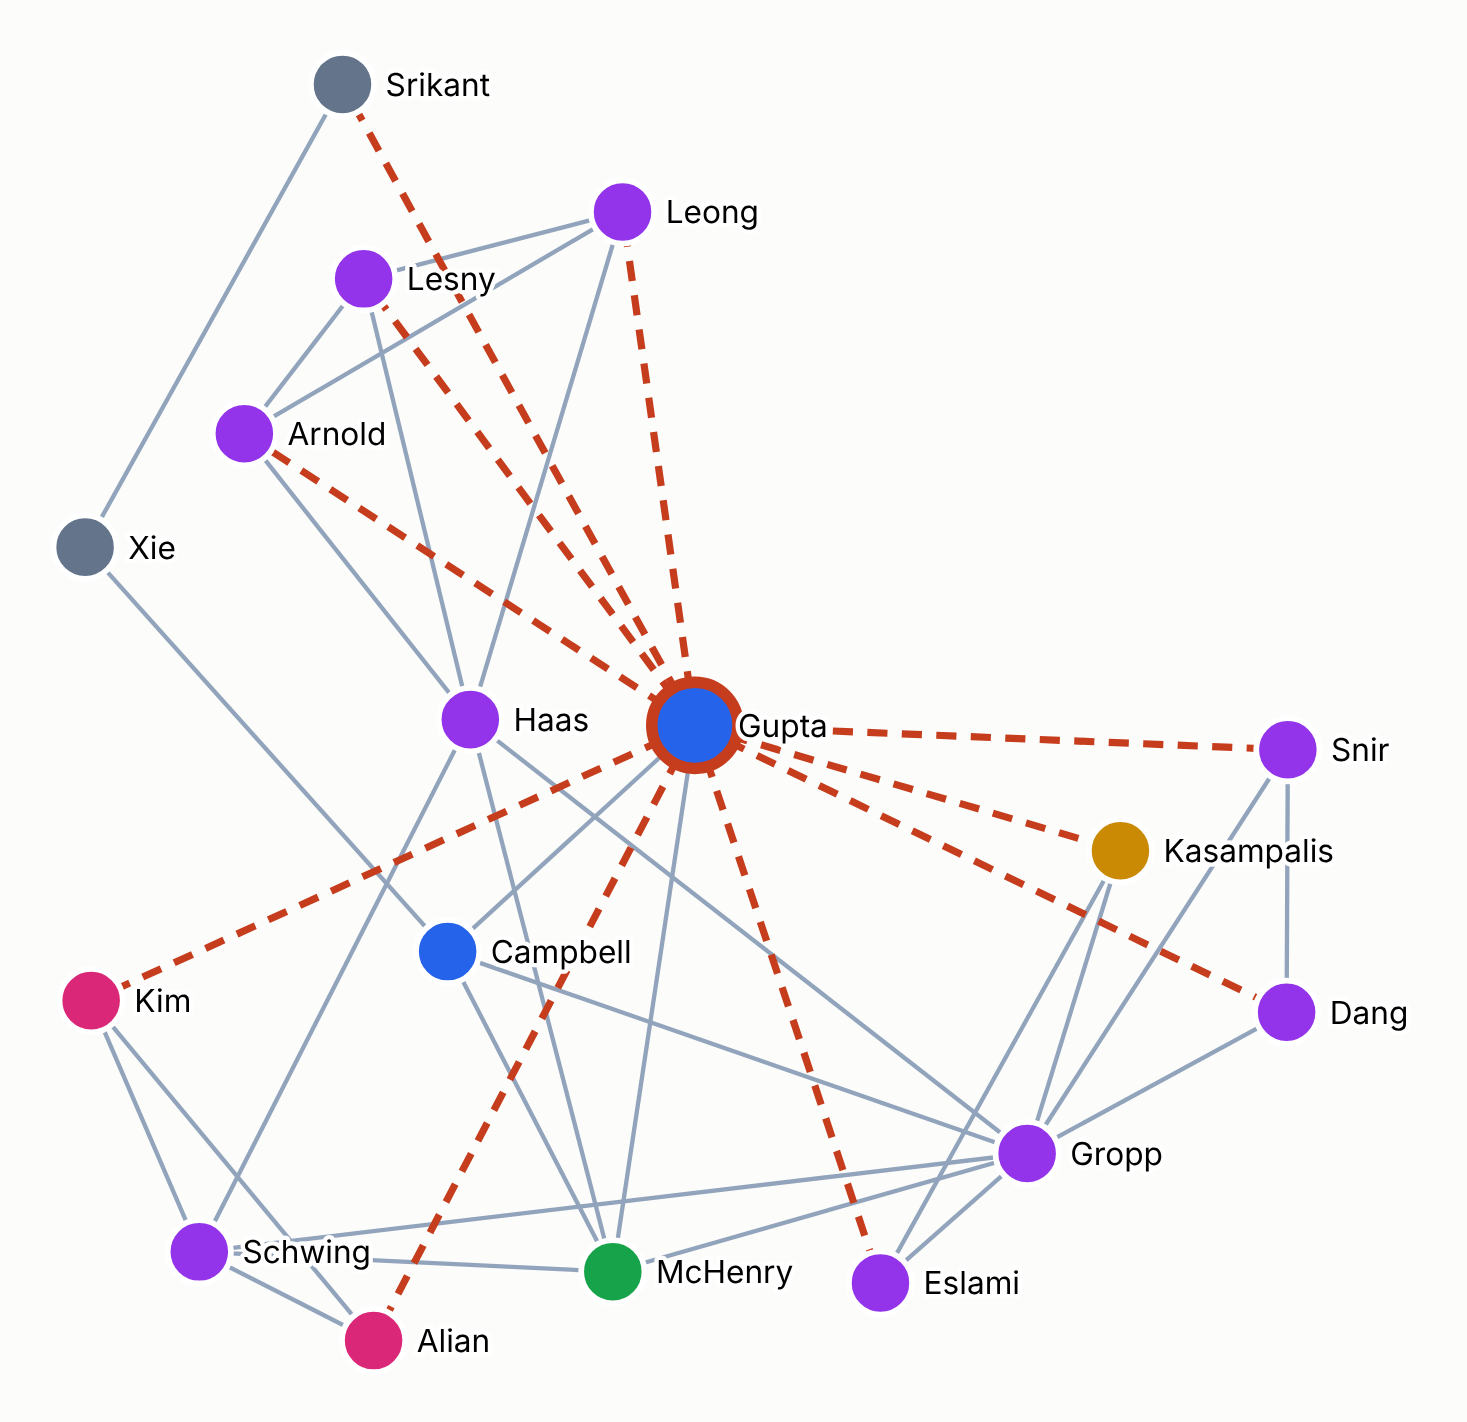
\includegraphics[width=0.62\textwidth,trim=0 150 0 0,clip]{midterm/review/screenshots/02-map.png}\\[3pt]
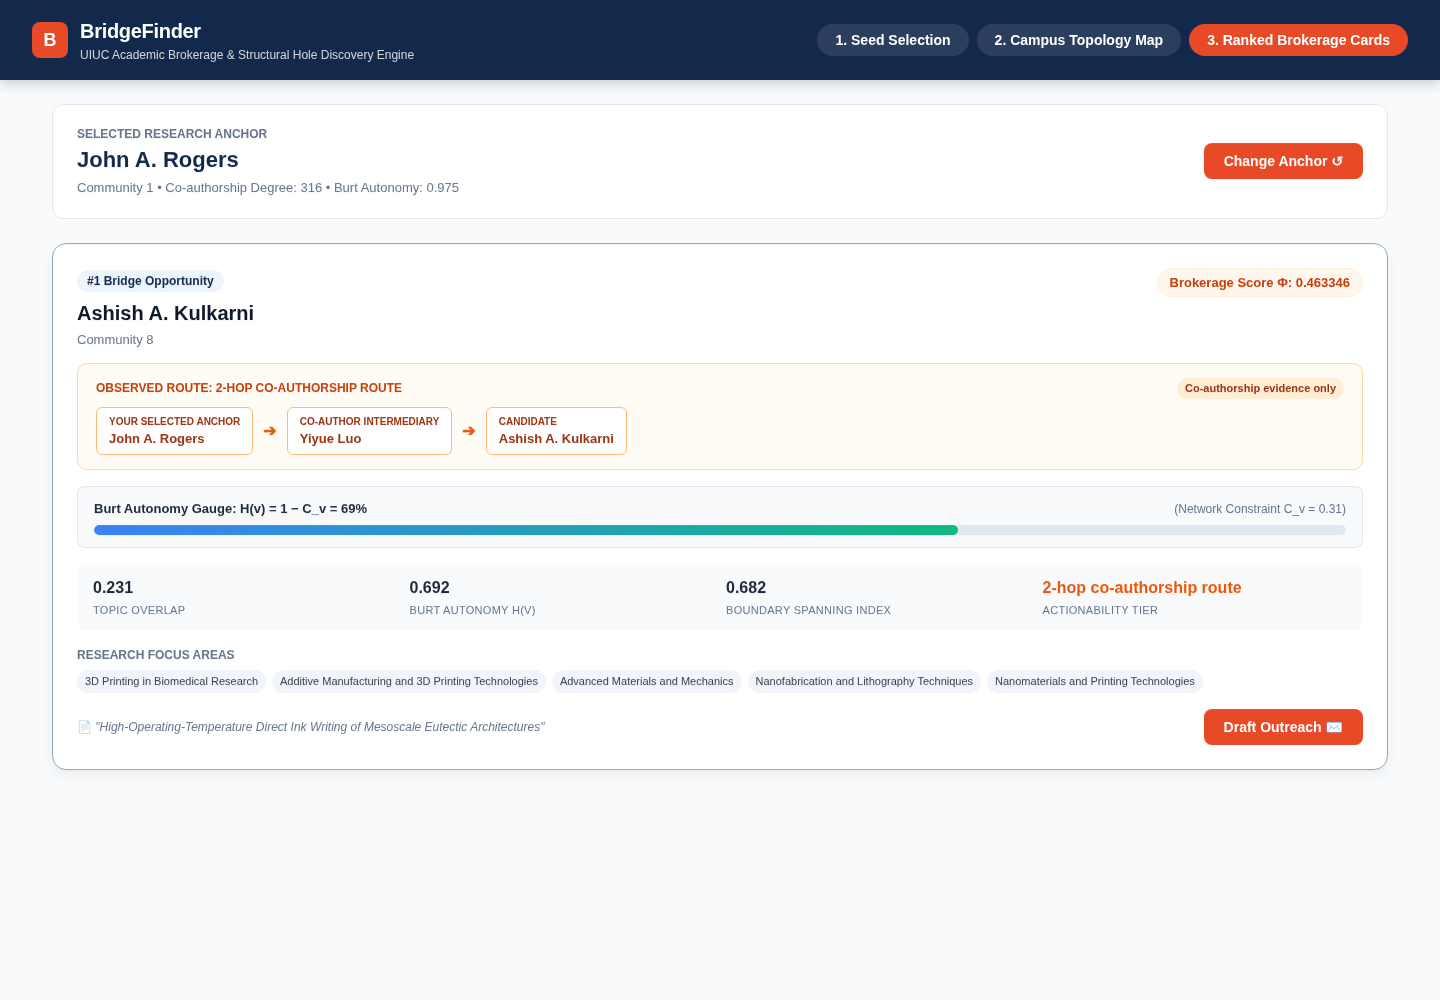
\includegraphics[width=0.82\textwidth,trim=45 205 45 205,clip]{midterm/review/screenshots/03-recommendation.png}
\caption{Implemented prototype. Top: selecting John A. Rogers shows cross-community suggestions; solid lines are observed co-authorships and dashed orange lines are suggested collaborations. Bottom: Ashish A. Kulkarni's card shows a possible route through Yiyue Luo, topics, and example papers. A publication path does not guarantee an introduction.}
\label{fig:prototype}
\end{figure*}

\subsection{What works now}
Python computes recommendations in advance, and a static D3 web page displays them. The app, prediction test, and study cards share graph and ranking code, keeping the evaluation aligned with the interface.

Cards show only observed paths, with at most two intermediaries, and explicitly mark unavailable routes. An outreach button opens an editable message without sending email. Automated checks verify rankings and route edges, and a browser walkthrough confirms that the main flow works. The next user round will test whether people understand it.

\section{Users and Feedback}
Our target users are UIUC students who want research opportunities beyond their current department. They may know a subject through classes but have few research contacts. We gathered feedback from five students in individual, 30-minute sessions, during which they talked through the early prototype: three CS/CE undergraduate juniors or seniors and two graduate students from Bioengineering and Information Sciences.

This mix is useful for an initial design round. The undergraduates represent the app's entry problem: exploring research before having publications of their own. Including graduate students in application areas brings another perspective on interpreting unfamiliar research and contacts. Five sessions allow close attention to interaction problems~\cite{nielsen1993}; they do not support a campus-wide estimate of usability. The purpose of this round was to improve the main flow before comparing recommendation quality with a broader sample.

The feedback led to three changes, each addressing a different point in that flow:

\textbf{Getting started.} Students without publications could not use themselves as the starting node. We added the searchable researcher list, so a familiar instructor can provide an entry point. This avoids requiring a new student to have an academic profile before using the app.

\textbf{Reading the map.} Students interpreted dashed lines as weak existing collaborations. We added a legend separating observed co-authorship from suggested connections. The distinction is visible in the map in Figure~\ref{fig:prototype}: dashed links identify candidates to explore, not relationships that already exist.

\textbf{Choosing a next step.} Students looked for who might introduce them before reading papers and topics. They also read a low constraint score as a poor recommendation. We moved the route to the top of the card and showed autonomy as a positive gauge. The card in Figure~\ref{fig:prototype} shows the resulting order: introduction first, then scores, topics, and example work.

These observations explain the design changes, but do not show that the changes solved the problems. In the next round, students will explain the line types and suggested route without help, allowing us to check comprehension rather than infer it from successful clicks. We report these first-round findings qualitatively, without issue frequencies or participant quotations.

\section{Evaluation}
\subsection{Prediction test}
We built the graph and topic profiles using only 2015--2019 papers, then asked whether the recommended researchers actually became new cross-community co-authors in 2020--2024. We evaluated 180 starting researchers in the pilot sample and 1,385 in the larger sample. Each had at least one eligible new collaboration in the later period. This excludes researchers who formed no such ties, so the results do not describe every researcher or student.

All methods rank the same candidates. Topic-Only tests whether topic matching is enough; Adamic--Adar tests shared contacts. Preferential attachment favors well-connected researchers, and betweenness favors researchers who lie on many shortest paths. Topic+Path tests a simpler version of our model.

We report \textbf{precision at five (P@5)}, the fraction of the first five suggestions that became collaborators, because students should not have to inspect a long list. We also report \textbf{NDCG@10}, which gives more credit when actual collaborators appear near the top of the first ten results. Both are averaged across starting researchers. Table~\ref{tab:results} reports the current implementation's results.

\begin{table}[!ht]
\centering\small
\setlength{\tabcolsep}{3pt}
\caption{Prediction of new 2020--2024 cross-community collaborations. Higher values are better.}
\label{tab:results}
\renewcommand{\arraystretch}{1.12}
\begin{tabularx}{\columnwidth}{@{}Xrr@{\hspace{9pt}}rr@{}}
\toprule
&\multicolumn{2}{c}{Pilot}&\multicolumn{2}{c}{Larger sample}\\
\cmidrule(lr){2-3}\cmidrule(l){4-5}
Method&P@5&\shortstack{NDCG\\@10}&P@5&\shortstack{NDCG\\@10}\\
\midrule
Pref. attachment&0.0011&0.0011&0.0088&0.0133\\
Betweenness&0.0011&0.0211&0.0078&0.0148\\
Topic-Only&0.0044&0.0274&0.0208&0.0402\\
Adamic--Adar&0.0056&0.0297&0.0295&0.0515\\
Topic+Path&0.0133&0.0615&0.0344&0.0620\\
BridgeFinder&0.0133&0.0514&0.0351&0.0674\\
\bottomrule
\end{tabularx}
\end{table}

On the larger sample, BridgeFinder improves P@5 from 0.0295 to 0.0351 over Adamic--Adar, a relative gain of about 19\%. NDCG@10 rises from 0.0515 to 0.0674. However, this falls short of our targets of doubling P@5 and adding 0.05 to NDCG@10. Precision is also low in absolute terms: only about 3.5\% of the top-five suggestions become observed collaborators.

\noindent\begin{minipage}{\columnwidth}
The simpler Topic+Path model has the same pilot P@5 as BridgeFinder and better pilot NDCG@10, while the full model performs better on the larger sample. The added features therefore do not help consistently. We have not yet estimated uncertainty around these differences. The results suggest that network information is useful, but do not establish reliable gains across settings or show that the app helps students find mentors.
\par
\end{minipage}

\subsection{Citation impact}
We also compared later papers involving authors from different training communities with papers whose known authors were in one community. This analysis separately excludes papers with more than 25 retained UIUC authors to reduce the influence of large teams.

Of 6,231 later papers, 1,071 were cross-community, 4,183 were within-community, and 977 could not be classified because none of their authors appeared in the training graph. Mean citations were 64.86 and 61.60, respectively, a ratio of 1.053. The medians were 36 and 37. A two-sided Mann--Whitney test gave $p=0.0601$.

Our target was a mean ratio above 1.10 and a statistically significant distributional difference ($p<0.05$); neither was met. This test also does not account for field, publication age, or repeated teams. We therefore cannot conclude that crossing communities leads to more influential work.

\subsection{Student evaluation}
The next round will recruit 15 students, aiming for three each from CS, ECE, Bioengineering, Crop Sciences, and Information Sciences. This broadens the first round beyond computing. It remains an exploratory study, not a representative campus survey.

Each participant will first use the app to find a candidate and explain the suggested route. They will then choose a starting researcher and rate up to 15 shuffled cards: the top five from BridgeFinder, Adamic--Adar, and Topic-Only. Method labels will be hidden. A candidate selected by more than one method will appear once, with the rating counted for each method that selected it.

We will measure three kinds of success:
\begin{itemize}
\setlength{\itemsep}{2pt}
\item \textbf{Relevance and discovery.} Participants rate relevance and novelty from 1 to 7. We target mean scores of at least 5 for each. Our main comparison is the share of cards rated at least 5 on both scales: BridgeFinder should exceed Adamic--Adar by 25 percentage points. Topic-Only provides a second comparison.
\item \textbf{Willingness to act.} Participants rate how realistic it feels to contact the candidate, also from 1 to 7. We target at least 5 and an improvement over Topic-Only, testing whether the path adds practical value.
\item \textbf{Usability and understanding.} At least 12 of 15 participants should complete the task without help and correctly distinguish observed ties from suggested connections. We will also use the standard ten-question System Usability Scale (SUS), targeting a mean of at least 80 out of 100.
\end{itemize}
We will compare methods using each participant's average ratings, rather than treating all cards as independent observations. The main joint relevance-and-novelty comparison will use a paired Wilcoxon test at $p<0.05$, with differences and uncertainty intervals reported. Other comparisons will be exploratory and use Holm correction for multiple tests. The rating interface, SUS questionnaire, export, and analysis scripts are implemented and tested. The comparative study itself has not yet been run.

\section{Limitations and Next Steps}
A publication path cannot tell us whether someone currently takes students or would make an introduction. Our historical UIUC sample also misses informal relationships, external collaborators, and some publications. The prediction gains therefore need to be tested against students' actual experience of the app.

In November, we will run the 15-student study and revise the interface. Any scoring changes will use separate validation data. The final report will combine user findings and prediction results to assess whether BridgeFinder helps students choose useful contacts.

\section*{Contributions and AI Use}
Evan Lin worked on data collection, the prediction test, and the campus map. Eric Liu worked on scoring, citation analysis, study tools, and the formative sessions. Both contributed to the report. Claude assisted with early development and drafting; OpenAI Codex assisted with implementation checks, tests, and report revision. No participant responses or quotations were generated.

\begin{thebibliography}{99}\small\raggedright
\setlength{\itemsep}{1.2pt}\setlength{\parskip}{0pt}

\bibitem{blondel2008}
V.~D. Blondel, J.-L. Guillaume, R.~Lambiotte, and E.~Lefebvre.
\newblock Fast unfolding of communities in large networks.
\newblock {\em Journal of Statistical Mechanics: Theory and Experiment}, 2008(10):P10008, 2008.

\bibitem{burt1992}
R.~S. Burt.
\newblock {\em Structural Holes: The Social Structure of Competition}.
\newblock Harvard University Press, Cambridge, MA, 1992.

\bibitem{burt2004}
R.~S. Burt.
\newblock Structural holes and good ideas.
\newblock {\em American Journal of Sociology}, 110(2):349--399, 2004.

\bibitem{dahlander2013}
L.~Dahlander and D.~A. McFarland.
\newblock Ties that last: Tie formation and persistence in research collaborations over time.
\newblock {\em Administrative Science Quarterly}, 58(1):69--110, 2013.

\bibitem{girvan2002}
M.~Girvan and M.~E.~J. Newman.
\newblock Community structure in social and biological networks.
\newblock {\em Proceedings of the National Academy of Sciences}, 99(12):7821--7826, 2002.

\bibitem{granovetter1973}
M.~S. Granovetter.
\newblock The strength of weak ties.
\newblock {\em American Journal of Sociology}, 78(6):1360--1380, 1973.

\bibitem{libennowell2007}
D.~Liben-Nowell and J.~Kleinberg.
\newblock The link-prediction problem for social networks.
\newblock {\em Journal of the American Society for Information Science and Technology}, 58(7):1019--1031, 2007.

\bibitem{nielsen1993}
J.~Nielsen.
\newblock {\em Usability Engineering}.
\newblock Morgan Kaufmann, San Francisco, CA, 1993.

\bibitem{openalex}
J.~Priem, H.~Piwowar, and R.~Orr.
\newblock Openalex: A fully-open index of scholarly works, authors, venues, institutions, and concepts.
\newblock {\em arXiv preprint arXiv:2205.01833}, 2022.

\bibitem{tang2012}
J.~Tang, S.~Wu, J.~Sun, and H.~Su.
\newblock Cross-domain collaboration recommendation.
\newblock In {\em Proceedings of the 18th ACM SIGKDD International Conference on Knowledge Discovery and Data Mining (KDD '12)}, pages 1285--1293, 2012.

\bibitem{scholar}
Google.
\newblock Google Scholar: About.
\newblock \href{https://scholar.google.com/intl/en/scholar/about.html}{Google Scholar overview}.

\bibitem{connectedpapers}
Connected Papers.
\newblock Connected Papers: Explore connected papers in a visual graph.
\newblock \href{https://www.connectedpapers.com/}{connectedpapers.com}.

\bibitem{researchrabbit}
ResearchRabbit.
\newblock ResearchRabbit: Literature discovery.
\newblock \href{https://www.researchrabbit.ai/}{researchrabbit.ai}.

\bibitem{experts}
University~of Illinois.
\newblock Illinois experts: Research and scholarship at {UIUC}.
\newblock \href{https://experts.illinois.edu/}{experts.illinois.edu}, 2024.

\end{thebibliography}
\end{document}
